\subsection{Visualization of object lists}




The published topics of Ground-Truth data and Camera-Calculation data will be subscribed. Each topic contains the ego vehicle data and the specific generated object list. In order to evaluate the object lists, the objects will be analyzed per frame. In RVIZ, the objects are represented by primitive figures with the help of marker messages. Figure \ref{fig:Nodes} shows the used topics and nodes. Rectangles represent topics and ellipses the called nodes. Moreover, tf is a package and controls the coordinate relationship of the ego vehicle.

\begin{figure}[thpb]
	\centering
	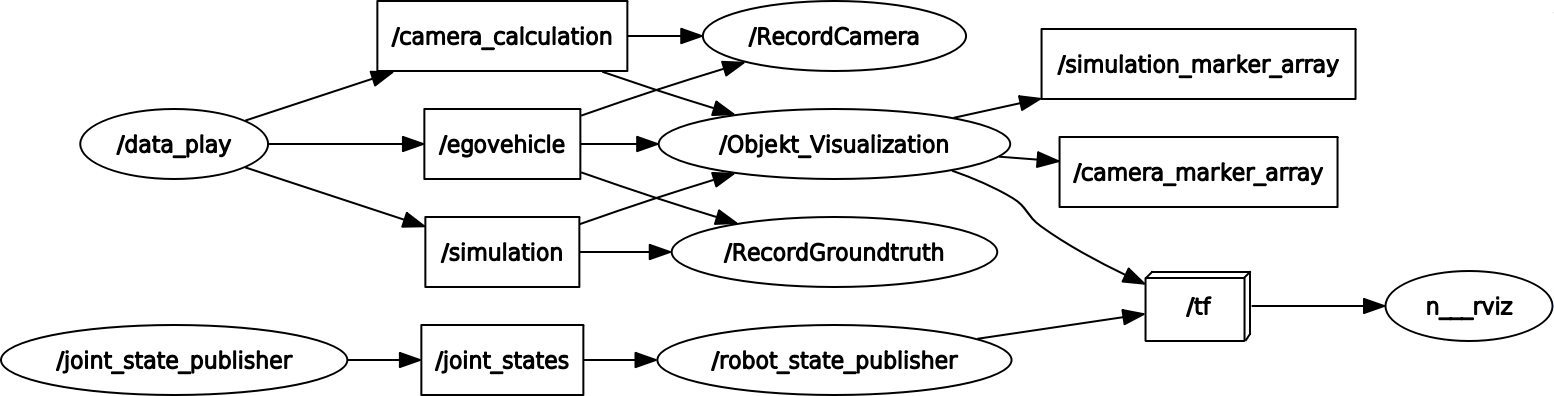
\includegraphics[width=\linewidth]{rosgraph}
	\caption{Nodes / Topics in ROS}
	\label{fig:Nodes}
\end{figure}



Marker messages are described with specific properties such as position, scale, type, color, orientation. Each object class will assigned selected shapes and colors so that they can be differentiate in RVIZ. The display variants for the possible object classes are shown in table \ref{ClassificationAssignment}. 

\begin{table}[h]
\caption{Classification Assignment}
\label{ClassificationAssignment}
\begin{center}
\begin{tabular}{c c c}
\hline
Classification & Shape & Color[RGB]\\
\hline
car & cube & [1, 0, 0]\\
truck & cube & [0, 1, 0]\\
pedestrian & cylinder & [0, 0, 1]\\
motorcyle & cube & [1, 0, 1]\\
car & cube & [1, 0, 0]\\
bicycle & cylinder & [1, 1, 0]\\
stacionary & sphere & [0, 1, 1]\\
other & sphere & [1, 1, 1]\\
\hline


\end{tabular}
\end{center}
\end{table}

In addition, the yaw angle of the objects has to be transformed into a quaternion for the visualization in RVIZ. The markers for the calculated camera data are assigned an RGB alpha value of 0.5, so that the difference between the camera data and the GT data is visually recognizable. 


The highest detection probability of an object indicates the classification, so that the properties value of each shape can assigned to the marker message. Furthermore, each detection position must be mirrored on the Y-axis, because the vehicle coordinate system does not match to the RVIZ coordinate system. Finally, the generated markers are combined into a marker array and will be published.

The ego vehicle is described as a robot model by a URDF model.
Furthermore, the model can be moved and rotated in the RVIZ coordinate system by tf messages. 

The pubished topics of Ground-Truth data, Camera-Calculation data and ego vehicle data are also saved in a Rosbag File. Each bagfile contains the published ego data and the corresponding object lists.In the following, these files are used for postprocessing.


